\begin{frame}[t]{The LHC Accelerator System}
\centering
\begin{columns}
\column{.5\textwidth}
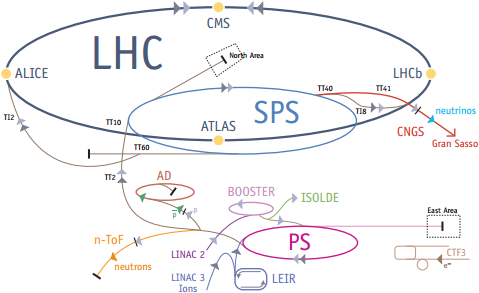
\includegraphics[width=.9\textwidth]{lhcb/lhc.png}

\column{.5\textwidth}
The main \lhc design parameters:
\resizebox{.9\textwidth}{!}{
\begin{tabular}{rr}\toprule
Circumference & 27\km\\
Center-of-mass energy & 14\tev\\
Injection energy & 450\gev\\
Field at 2 $\times$ 450\gev & 0.535\tesla\\
Field at 2 $\times$ 7\tev & 8\tesla\\
Helium temperature & 2\degk\\
Luminosity & $10^{34}\cm^{-2}s^{-1}$\\
Bunch spacing & 25\ns\\
Luminosity lifetime & 10\hr\\
Time between 2 fills & 7\hr\\
\bottomrule
\end{tabular}
}
\end{columns}
\bigskip
The \lhc operated mainly at center-of-mass energies of 7\tev and 8\tev in 2011
and 2012, respectively. In 2015, after the long  shutdown, \lhc is planned to
reach energy of 13\tev.
\end{frame}